The crucial part of the player engagement is the game’s design and its mechanics, which need to include elements that will motivate the player to play. Such elements are universal for any other game genre, as the play needs to be meaningful. Importantly, “The meaning of a game is facilitated by design: when players can choose among playing to win, playing to keep the game interesting, or playing to manage the social situation, a game quickly become socially meaningful” (Juul 2008: 22) \cite{casualrevolution}. Because rhythm games are a specific genre, they have their own unique elements that can be used to engage the player. Something that cannot be overlooked is the adaptation of rhythm games to the current playerbase and gaming market. Considering the meanings described by Juul, the player’s motivation may be as such:
\begin{itemize}
\item Playing to win -- Players are driven by the need to compete and improve their ranking, often facilitated by online leaderboards, achievements, and tournaments.
\item Playing to keep the game interesting -- Players are engaged by the opportunity to explore the various gamemodes, time-limited events, DLCs, or the option to create own mods and content for the community.
\item Playing to manage the social situation -- the player is motivated to play by the desire to socialize and connect with other players. This can be achieved through multiplayer modes, playing in arcade parks and community events.
\end{itemize}

This classification simplifies the various motivations that drive players, and it is important to note that these motivations often overlap and can influence one another. For example, a player may be motivated to play to win, but also enjoy the social aspect of competing with friends -- in such case the competetive aspect of the game may be countered by the motivation to spend quality time with friends. Additionally, the motivations can change over time, as players may become more interested in one aspect of the game as they progress or as the game evolves. The key is to create a game that offers a variety of experiences and allows players to engage with it in different ways, catering to their individual motivations and preferences.

\section{Playing to win -- the competitive aspect of rhythm games}
A simple scoring system naturally enables the desire to improve and compete with other players. The competitive aspect of rhythm games is often facilitated by online leaderboards -- showing best scores on the particular song and difficulty and the general ones that summarize all scores achieved. In many rhythm games, the leaderboard, which ranks players based on their highest all-time scores, lacks the element of real-time competition. Because of this, the players may be motivated to engage in tournaments that will allow them to compete with other players in real-time. Such tournaments may be organized by the developers or held unofficially by the community. Usually, the tournaments organized by the developers focus on the best players, while the community tournaments are more casual and focus on the fun of playing together, often including players from lower-rank brackets. Such form of play measures different skills than simply playing the game by itself, as it deprives the player from the ability to retry the song after missing a note or failing, which is a common practice in the single-player mode. In this setting, players are required to complete the song in a single attempt, which can be particularly challenging for those accustomed to repeating tracks multiple times to achieve a perfect score. Therefore, even if the tournament is held online, it takes a different form than competing for the best score on the leaderboard.
Taking \textit{osu! World Cup} as an example, the tournament is held in a country-based format, where players are divided into teams representing their countries. The tournament is played in a series of matches, where each match consists of a set of maps that both competing teams are playing simultaneously. There are two stages of the tournament: the Group Stage and the Knock-Out Stage. The Group Stage consists of a round-robin format, forming eight groups that consists of four teams, where each team plays a match against every other team in their group. In this stage, matches are played in best of 9 format, meaning that the first team to win 5 maps wins the match. Two best teams from each group advance to the Knock-Out stage, which is played in double-elimination bracket (winners and losers bracket). In the Knock-Out Stage, Quarterfinals are played in best of 11 format, while Semifinals, Finals and Grand Finals are played in best of 13 format.

\begin{figure}[h]
    \centering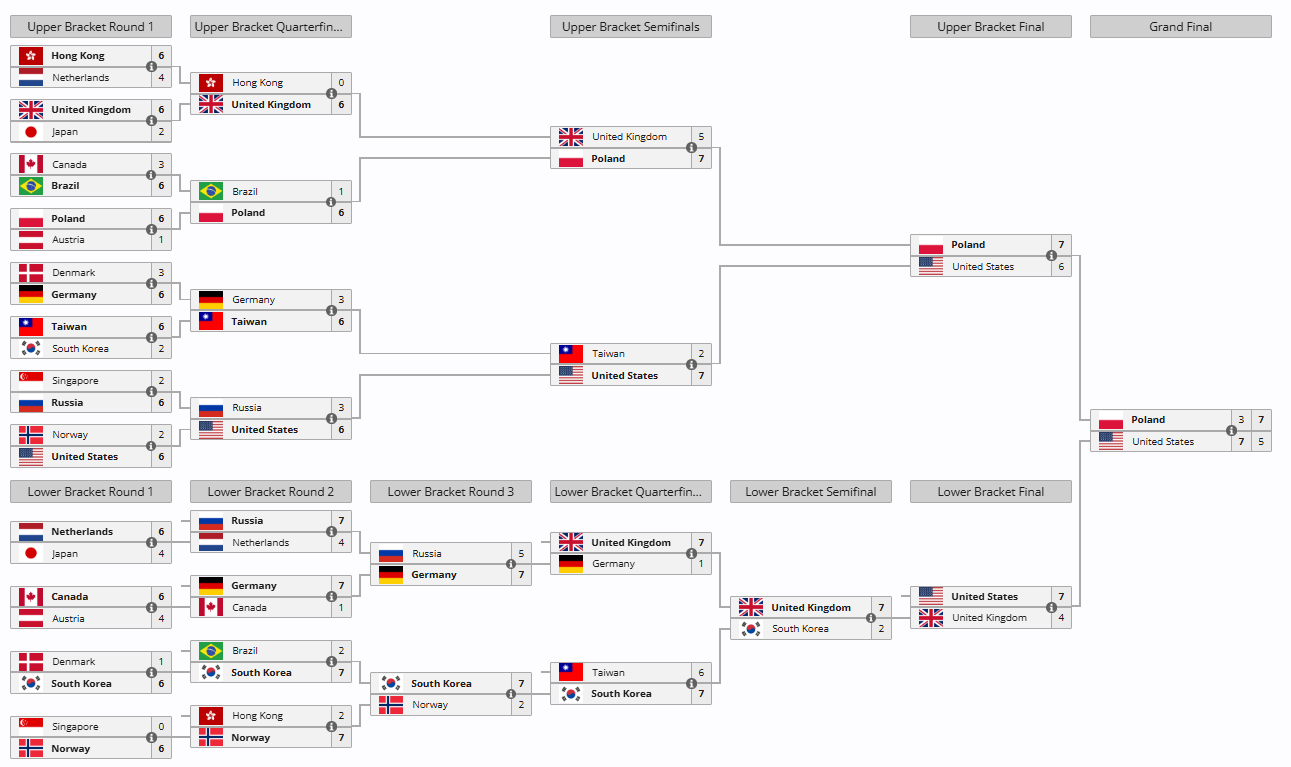
\includegraphics[scale=0.15]{obrazki/osuworldcup.png}
    \caption{\textit{osu! World Cup} -- upper and lower bracket of 2017 tournament. The teams that lost in the upper bracket are moved to the lower bracket, where they have a chance to continue playing and still compete for the first place. \cite{2017osu}}
    \label{fig:osuworldcup}
\end{figure}

During the match, teams take turns in picking the beatmap, which is then played by both teams. Each team is also allowed to ban a desired map, preventing their opponent from picking it. One round of the match represents a single playthrough of a beatmap. The scores from all four players on a team are added together to form the team’s score for that round. The team with the higher accumulated score wins the round, scoring a point for their team. The first team to win the required number of rounds wins the match. As the tournament is held online and its players are playing from home, the matches are streamed online, allowing the audience to watch it live.
Such form of tournament places the player in significantly different environment than regular, single-mode play. Because players are playing in a team, the tournament is not only about their individual skill, but also about the teamwork and communication between players - they must decide together how to approach the opposing team, what are their strengths and weaknesses or which maps should they practice more. As mentioned earlier, depriving the player from the ability to retry or pause the song makes the tournament more challenging, as the player must be prepared to play the song as best as they can in a single attempt. Managing the pressure of the livestreamed tournament is another challenge that the player must face. The skillset required to play in a tournament is different than the one required to play in a single-player mode, as the player must be able to perform well under pressure and adapt to the team’s needs. Even within the community, it's widely recognized that some players may not hold the top spot on the general leaderboard, yet they consistently outperform higher-ranked players when it comes to tournaments. One of such players is Maliszewski - a well-known \textit{osu!} player from Poland, who is recognized for his exceptional performance in tournaments, despite not being higher than 10th place on the global leaderboard. His success in tournaments can be attributed to his ability to perform well under pressure and adapt to the needs of his team. His example shows that the skillset required for tournament play is different than the one required for single-player mode \cite{maliszewski}.

\section{Playing to keep the game interesting -- outside the core gameplay}
As current gaming market makes the biggest profit from live service games, the genre of rhythm games adaptates this idea to its own needs. The live service model allows developers to keep the game fresh and engaging for players by regularly releasing new content, such as songs, gamemodes, and time-limited events. This solution assures to keep the player interest and encourage them to continue playing over time. In this case, rhythm game developers focus on releasing DLCs with new songs and extra difficulties, often including recently released songs from popular artists or franchises, such as Vocaloid. Additionally, many rhythm games also include time-limited events, which can create a sense of urgency and encourage players to log in and play regularly. For example, in arcade rhythm games such as \textit{maimai}, the player receives in-game currency for daily log-in from IC Card and completing current time-limited challenges. Additionally, the owner of the cab needs to update it regularly, as the developer continues to support the game and release the new updates with additional content. This solution is different than old-school arcades that were released once, completed on the day of the release as the new version came only alongside a completly new cab release. This day, as the cabs are connected to the internet, the new content is distributed online and arcade parks can easily update the game. Nowadays, the new cab is released only when the hardware of the old one is insufficient -- for example, \textit{maimai} continues to receive new updates only on the newer version of its arcade machine. The first generation of the cabinet received 12 updates between the year 2012 and 2019 before the introduction of the new mechanic: tap-notes, which needed the upgraded version of the touchscreen. The second generation of the arcade machine with upgraded touchscreen was released as \textit{maimai DX} in July 2019. Currently, the second generation of \textit{maimai DX} machines receives new updates once per few months. Between the releases, the playerbase receives time-limited events with missions, achievements, profile titles and cosmetics. 

\section{Playing to manage the social situation -- the culture of rhythm games and its community}
The social aspect of rhythm games is often overlooked, but it is an important part of the player experience. Many players enjoy playing rhythm games with friends or in a social setting, such as an arcade park or online multiplayer mode. As Alexander Chan highlights: “Throughout the history of video and computer games, game communities have often been as interesting to examine as the games themselves. They form an integral part of the entire game environment and without examining the game community, any exploration of a game would be incomplete” (Chan 2004: 6) \cite{arcadeculture} -- rhythm games are no exception. Early rhythm game communities formed in arcade parks, where players gathered locally in order to play on cabs. With the rise of PC rhythm games and the growth of online forums, these communities gradually transitioned to the internet. Today, the social aspect is further enhanced by social media, community platforms, and chatrooms, allowing players to share experiences and build connections, that further enhance the sense of belonging to the community. Since the early days of the genre, social interaction has played a key role, contributing to the development of a distinct culture around rhythm games. In the early stages, this culture was heavily influenced by japanese pop culture and platforms like NicoNicoDouga, which hosted a large volume of fan-made content that developers and players integrated into rhythm games. One example is the MAD video format—fan-made remixes that combine cutout fragments from existing videos of other media, such as anime, films, or advertisements, often featuring recognizable characters. One of the primarly example is a MAD video known as \textit{“Ronald McDonald Insanity”}, which is a remix of a song \textit{U.N. Owen Was Her?} from \textit{Touhou Project} -- featuring rapid cuts of Ronald McDonald from the McDonald’s commercials. The video was released in 2007 on NicoNicoDouga and quickly gained popularity, making its way into various rhythm games, including \textit{Stepmania} and \textit{osu!}. Inrestingly, \textit{Touhou Project} music and its fan-made content is commonly featured in rhythm games. The popularity of \textit{Touhou Project} music in rhythm games can be attributed to the fact that the franchise has a large and diverse library of songs, which are often remixed and rearranged by its talented and creative fans. The community-driven nature of rhythm games and their intersection with other fandoms have also contributed to the popularity of other forms of media, such as Vocaloid -- voice-synthesizing software used to create songs, often featuring virtual singers, such as Hatsune Miku, the most popular one. Rhythm games, especially \textit{Hatsune Miku: Project Diva} series, played a significant role in popularizing Vocaloid music globally introducing it to the larger audience. Overall, the social aspect of rhythm games is a crucial part of the player experience, as it allows players to not only connect with others, but also creates an opportunity to interact with other media and find new interests.

\section{Engagement through embodied play}
Outside the player's motivation described by Juul, the unique aspect of the rhythm game's genre is the physicality of the play. In case of arcade rhythm games, the player is required to use their body to play the game, which creates a different experience from the traditional play. The study \textit{Get in the Game The influence of embodied play on presence and flow in videogames} shows the relevance of embodiment in video games and its relation to flow state. 